\section{Wireshark Packet Capture and Protocol Analysis}
\label{sec:wireshark_analysis}

Addressing Rubric Section~III (\qty{15}{\percent}), this section presents the empirical Deep Packet Inspection (DPI) of live HTTPS communications traversing the ZeroTier Software-Defined Wide Area Network (SD-WAN) between Universidad de los Llanos and the Seneca Polytechnic gateway node. Using Wireshark's protocol dissector~\cite{wireshark2023}, the capture verifies three operational invariants across the encrypted overlay tunnel: (i)~interface-calibrated TCP three-way synchronization~\cite{rfc9293,kozierok2005}, (ii)~single-round-trip (1-RTT) TLS~1.3 cryptographic negotiation and encrypted HTTP/1.1 payload delivery~\cite{rfc8446,tanenbaum2021}, and (iii)~orderly four-way TCP connection teardown free of abnormal resets.

\subsection{Capture Environment and Compliance Metadata}
\label{subsec:pcap_metadata}

Live traffic was intercepted directly on the ZeroTier virtual network adapter (\texttt{\textbackslash{}Device\textbackslash{}NPF\_\allowbreak\{447C8263-\allowbreak DE63-\allowbreak 4294-\allowbreak AF23-\allowbreak 24A2B16FBE83\}}, interface alias \texttt{ZeroTier One [abfd31bd47affa39]}) while requesting the Seneca Polytechnic cultural intranet from the UniLlanos host (\nolinkurl{172.22.201.2}) toward the Seneca simulated server (\nolinkurl{172.22.31.69}) on TCP port~443. The resulting trace, archived at \nolinkurl{modulo2/wireshark/coil_sdwan_https_traffic.pcapng}, occupies \qty{25408}{\byte} (\qty{24.81}{\kilo\byte}), remaining strictly below the \qty{10}{\mega\byte} rubric ceiling at just \qty{0.24}{\percent} of the maximum file-size budget.

Across the complete trace, Wireshark recorded \num{44} frames (\qty{23451}{\byte} captured on wire). Protocol Hierarchy Statistics (PHS) partition these \num{44} frames into two Layer-4 trees:
\begin{itemize}
    \item \textbf{UDP Tree (\num{8} frames):} Comprises \num{7} Domain Name System (DNS) frames~\cite{rfc1035} and \num{1} local overlay broadcast datagram. Notably, Frames~1--2 capture the initial SD-WAN DNS resolution over UDP port~53 in \qty{0.0005346}{\second} (\qty{0.5346}{\milli\second}), resolving \nolinkurl{www.coil-group2.com} to \nolinkurl{172.22.201.2} immediately prior to TCP connection setup; the dedicated DNS capture screenshot (\nolinkurl{wireshark_5_dns_resolution.png}) and its query/response dissection are presented in Manual~4 of Rubric Section~IV to avoid visual duplication.
    \item \textbf{TCP Tree (\num{36} frames, \qty{22785}{\byte} on wire):} Captures the single bidirectional HTTPS conversation \nolinkurl{172.22.201.2:52382 <-> 172.22.31.69:443} over a duration of \qty{0.4083}{\second} (\qty{0.2392395}{\second} to \qty{0.6475791}{\second}), carrying dissected \texttt{TLSv1.3} encrypted records with zero TCP retransmissions, zero out-of-order segments, and zero \texttt{RST} flags.
\end{itemize}

Table~\ref{tab:pcap_metadata} consolidates the quantitative capture metadata, directional TCP byte counters, and rubric compliance indicators extracted from the trace.

\begin{table}[t]
\centering
\caption{Wireshark Capture Compliance Metadata and Bidirectional HTTPS Flow Metrics.}
\label{tab:pcap_metadata}
\footnotesize
\setlength{\tabcolsep}{4pt}
\renewcommand{\arraystretch}{1.18}
\begin{tabularx}{\columnwidth}{@{} >{\bfseries\raggedright\arraybackslash}p{2.65cm} >{\raggedright\arraybackslash}X @{}}
\toprule
Parameter & Measured Value / Verification Result \\
\midrule
Capture Artifact & \nolinkurl{modulo2/wireshark/coil_sdwan_https_traffic.pcapng} \\
Capture Interface & \texttt{\textbackslash{}Device\textbackslash{}NPF\_\allowbreak\{447C8263-\allowbreak DE63-\allowbreak 4294-\allowbreak AF23-\allowbreak 24A2B16FBE83\}} (\texttt{ZeroTier One [abfd31bd47affa39]}) \\
File Size & \qty{25408}{\byte} (\qty{24.81}{\kilo\byte}); strictly $< \qty{10}{\mega\byte}$ (\qty{0.24}{\percent} of budget) \\
Total Trace Frames & \num{44} frames (\qty{23451}{\byte} captured on wire) \\
Protocol Hierarchy & UDP: \num{8} frames (DNS: \num{7} frames, incl.\ Frames~1--2 at \qty{0.0005346}{\second}); TCP: \num{36} frames (\texttt{TLSv1.3} record dissection) \\
Filtered HTTPS Flow & \nolinkurl{172.22.201.2:52382 <-> 172.22.31.69:443} (\num{36} frames, \qty{22785}{\byte} wire, \qty{0.4083}{\second} duration) \\
Client Contribution & \num{15} frames / \qty{2505}{\byte} wire / \qty{1684}{\byte} TCP payload \\
Server Contribution & \num{21} frames / \qty{20}{\kilo\byte} wire / \qty{19135}{\byte} TCP payload \\
Transport Anomalies & \num{0} retransmissions, \num{0} lost segments, \num{0} \texttt{RST} flags \\
\bottomrule
\end{tabularx}
\end{table}

\subsection{Display Filter Isolation of the Partner HTTPS Flow}
\label{subsec:ws_display_filter}

Because virtual overlay adapters simultaneously carry background discovery broadcasts and host-level DNS probes (such as the \num{8} UDP frames present in the unfiltered buffer), raw capture views obscure transport-layer state transitions. Applying the boolean Wireshark display filter in Listing~\ref{lst:ws_display_filter} restricts visualization strictly to packets matching the Seneca server address and HTTPS destination/source port~\cite{wireshark2023}.

\begin{lstlisting}[caption={Wireshark display filter isolating the UniLlanos--Seneca HTTPS conversation.}, label={lst:ws_display_filter}, numbers=none, xleftmargin=0pt, framexleftmargin=0pt]
ip.addr == 172.22.31.69 and tcp.port == 443
\end{lstlisting}

As shown in Fig.~\ref{fig:ws_filtered}, this filter isolates all \num{36} frames (Frames~3--38, representing \qty{22785}{\byte} on wire) belonging to the \texttt{172.22.201.2:52382} $\leftrightarrow$ \texttt{172.22.31.69:443} TCP stream while suppressing both the preceding SD-WAN DNS frames (Frames~1--2) and subsequent background UDP traffic (Frames~39--44). The packet list pane confirms clean chronological progression across connection setup, TLS~1.3 cryptographic exchange, full HTML payload streaming, and graceful teardown within \qty{0.4083}{\second}.

\begin{figure*}[t]
    \centering
    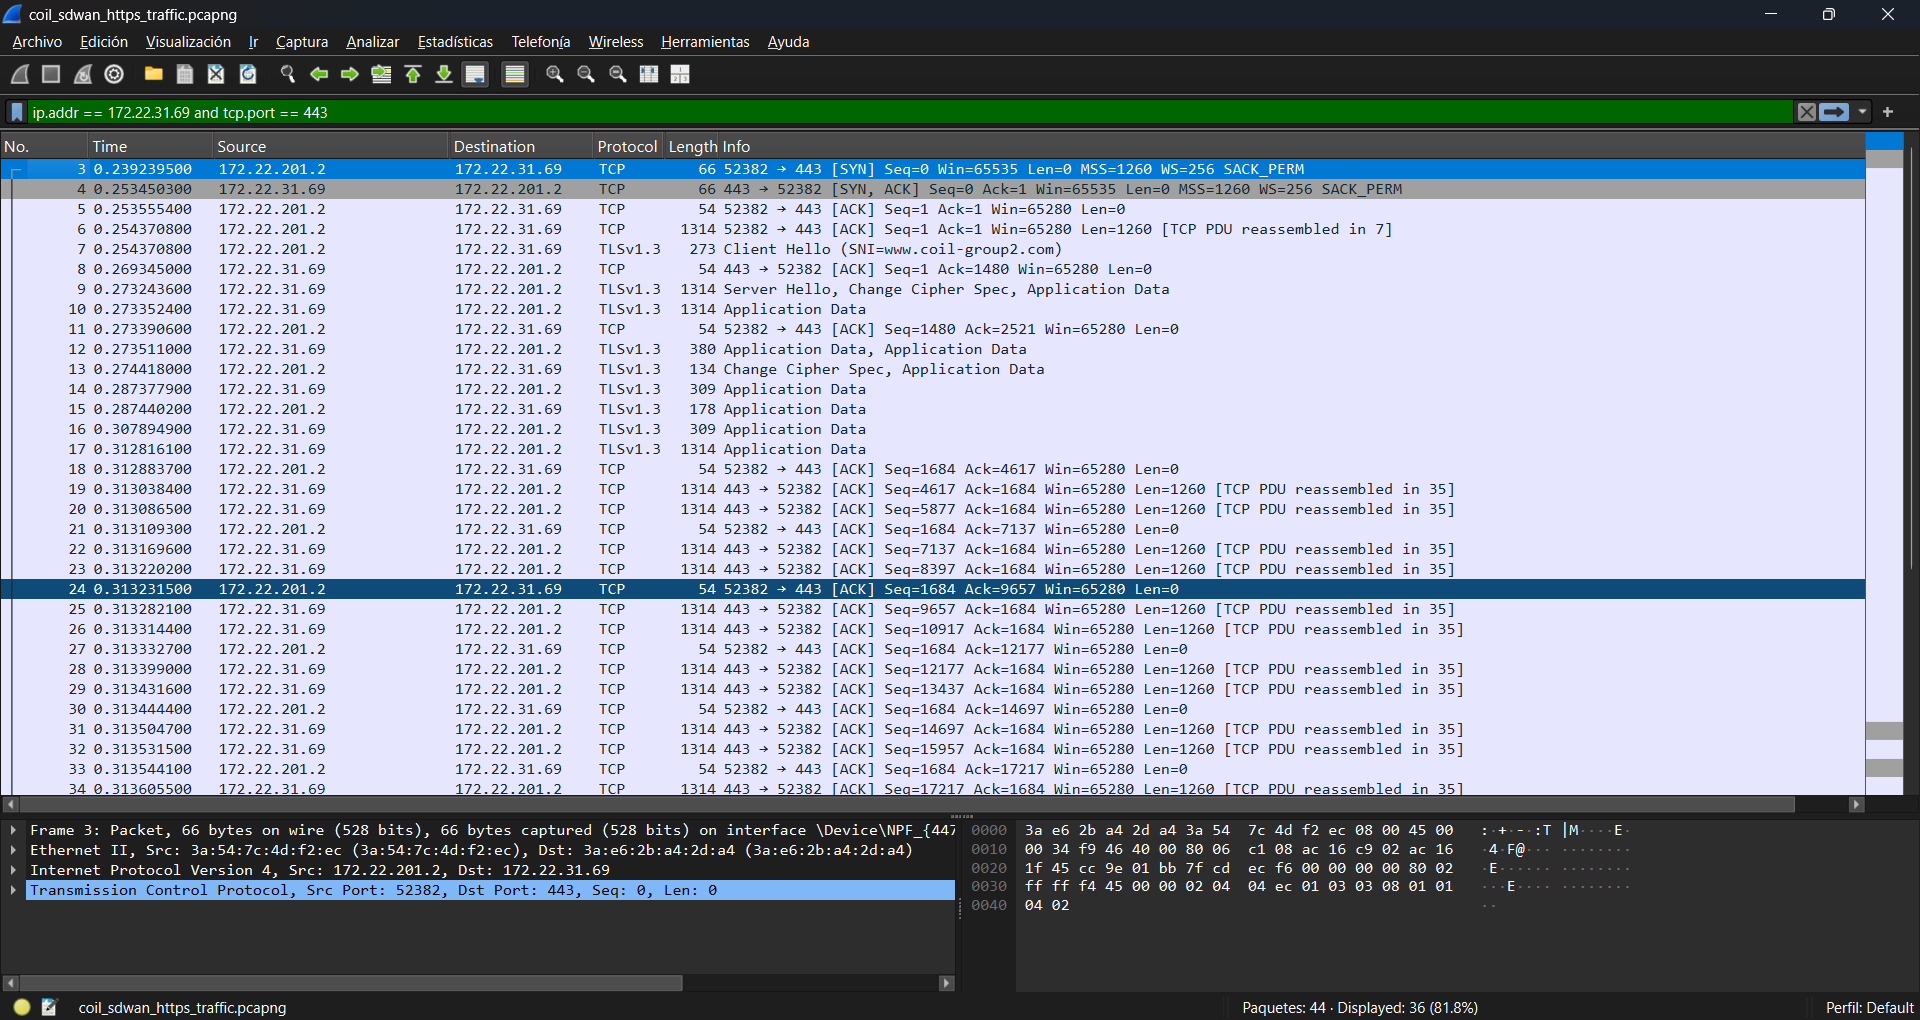
\includegraphics[width=0.94\textwidth]{figuras/wireshark_1_filtered_traffic.png}
    \caption{Wireshark packet list with the display filter \texttt{ip.addr == 172.22.31.69 and tcp.port == 443} applied, isolating all \num{36} frames (\qty{22785}{\byte} wire, \qty{0.4083}{\second} duration) of the HTTPS conversation between UniLlanos (\nolinkurl{172.22.201.2:52382}) and Seneca (\nolinkurl{172.22.31.69:443}).}
    \label{fig:ws_filtered}
\end{figure*}

To map the wire-level packet stream onto its protocol state transitions before examining individual dissection panes, Fig.~\ref{fig:tcp_tls_sequence} synthesizes the complete end-to-end packet sequence diagram across TCP handshake, TLS~1.3 record exchange, segmented HTTP/1.1 response delivery, and four-way termination. The subsections that follow corroborate each phase in Fig.~\ref{fig:tcp_tls_sequence} directly against the corresponding Wireshark captures (Figs.~\ref{fig:ws_handshake}--\ref{fig:ws_teardown}).

\begin{figure*}[htbp]
\centering
\resizebox{0.84\textwidth}{!}{%
\begin{tikzpicture}[
    >=Stealth,
    every node/.style={font=\scriptsize, text=black!88},
    /utils/exec={
        \definecolor{figTwoSlate}{HTML}{1E293B}
        \definecolor{figTwoMuted}{HTML}{475569}
        \definecolor{figTwoRule}{HTML}{CBD5E1}
        \definecolor{figTwoDnsAccent}{HTML}{0F766E}
        \definecolor{figTwoDnsFill}{HTML}{F0FDFA}
        \definecolor{figTwoDnsBadge}{HTML}{CCFBF1}
        \definecolor{figTwoTcpAccent}{HTML}{1D4ED8}
        \definecolor{figTwoTcpFill}{HTML}{EFF6FF}
        \definecolor{figTwoTcpBadge}{HTML}{DBEAFE}
        \definecolor{figTwoTlsAccent}{HTML}{6D28D9}
        \definecolor{figTwoTlsFill}{HTML}{F5F3FF}
        \definecolor{figTwoTlsBadge}{HTML}{EDE9FE}
        \definecolor{figTwoDataAccent}{HTML}{047857}
        \definecolor{figTwoDataFill}{HTML}{ECFDF5}
        \definecolor{figTwoDataBadge}{HTML}{D1FAE5}
        \definecolor{figTwoFinAccent}{HTML}{B45309}
        \definecolor{figTwoFinFill}{HTML}{FFFBEB}
        \definecolor{figTwoFinBadge}{HTML}{FEF3C7}
    },
    endpoint/.style={
        rectangle, rounded corners=3pt, draw=figTwoSlate, fill=white,
        line width=0.9pt, align=center, inner xsep=4pt, inner ysep=5pt,
        minimum height=1.24cm, font=\scriptsize
    },
    endpoint_foot/.style={
        rectangle, rounded corners=2.5pt, draw=figTwoSlate, fill=figTwoSlate!6,
        line width=0.7pt, align=center, inner xsep=4pt, inner ysep=3.5pt,
        font=\scriptsize\bfseries, text=figTwoSlate
    },
    phase_badge/.style={
        rectangle, rounded corners=2.5pt, align=center,
        text width=1.46cm, inner xsep=3pt, inner ysep=4.5pt,
        line width=0.7pt, font=\scriptsize\bfseries
    },
    telemetry_card/.style={
        rectangle, rounded corners=3pt, align=left,
        text width=5.35cm, inner xsep=6pt, inner ysep=5pt,
        line width=0.65pt, fill=white, font=\scriptsize
    },
    msg_arrow/.style={
        -{Stealth[length=5pt 1.2, width'=0pt 0.65]},
        line width=0.85pt, shorten >=1.5pt, shorten <=1.5pt
    },
    msg_burst/.style={
        -{Stealth[length=6pt 1.2, width'=0pt 0.65]},
        line width=1.5pt, shorten >=1.5pt, shorten <=1.5pt
    },
    msg_ack/.style={
        -{Stealth[length=4.5pt 1.1, width'=0pt 0.6]},
        line width=0.7pt, dashed, shorten >=1.5pt, shorten <=1.5pt
    },
    msg_label/.style={
        anchor=south, yshift=2.2pt, align=center, inner sep=1pt,
        font=\scriptsize, text=figTwoSlate
    },
    lifeline/.style={
        dashed, line width=0.75pt, color=figTwoMuted!65
    }
]

\node[endpoint, text width=2.95cm, fill=figTwoTcpFill!65, draw=figTwoTcpAccent] (client_hdr) at (0,0) {%
    \textbf{\color{figTwoTcpAccent}UniLlanos Client Host}\\[2pt]
    \texttt{172.22.201.2:52382}\\[2pt]
    {\tiny\color{figTwoMuted}TLS 1.3 / HTTPS Client}%
};

\node[endpoint, text width=3.40cm, fill=figTwoSlate!5, draw=figTwoSlate, right=3.45cm of client_hdr] (server_hdr) {%
    \textbf{\color{figTwoSlate}Seneca Gateway}\\[2pt]
    \texttt{172.22.31.69}\\[2pt]
    {\tiny\color{figTwoMuted}HTTPS :443 \textbar{} DNS Client :51420}%
};

\node[endpoint, text width=2.85cm, fill=figTwoDnsFill!75, draw=figTwoDnsAccent, right=1.95cm of server_hdr] (dns_hdr) {%
    \textbf{\color{figTwoDnsAccent}UniLlanos Auth DNS}\\[2pt]
    \texttt{172.22.201.2:53}\\[2pt]
    {\tiny\color{figTwoMuted}\texttt{dns\_server.py} (UDP)}%
};

\node[left=0.22cm of client_hdr, minimum width=1.64cm, minimum height=1.24cm, inner sep=0pt] (phase_hdr_anchor) {};
\node[align=center, font=\scriptsize\bfseries, text=figTwoMuted] at (phase_hdr_anchor.center) {Protocol\\[2pt]Phase};

\coordinate (hdr_mid) at ($(phase_hdr_anchor.north west)!0.5!(dns_hdr.north east)$);
\node[anchor=south, font=\small\bfseries, text=figTwoSlate, inner sep=2pt] (fig_title) at ($(hdr_mid)+(0,0.42)$)
    {SD-WAN DNS, TCP, and TLS 1.3 Sequence (38 Frames)};

\coordinate (t_start) at (phase_hdr_anchor.south);

\coordinate (r_p0_top)  at ($(t_start)+(0,-0.38)$);
\coordinate (r_f1)      at ($(r_p0_top)+(0,-0.88)$);
\coordinate (r_f2)      at ($(r_f1)+(0,-1.05)$);
\coordinate (r_dns_end) at ($(r_f2)+(0,-0.58)$);
\coordinate (r_p0_bot)  at ($(r_dns_end)+(0,-0.52)$);

\coordinate (r_p1_top)  at ($(r_p0_bot)+(0,-0.22)$);
\coordinate (r_f3)      at ($(r_p1_top)+(0,-0.88)$);
\coordinate (r_f4)      at ($(r_f3)+(0,-1.02)$);
\coordinate (r_f5)      at ($(r_f4)+(0,-0.78)$);
\coordinate (r_p1_bot)  at ($(r_f5)+(0,-0.32)$);

\coordinate (r_p2_top)  at ($(r_p1_bot)+(0,-0.22)$);
\coordinate (r_f6)      at ($(r_p2_top)+(0,-0.92)$);
\coordinate (r_f9)      at ($(r_f6)+(0,-1.10)$);
\coordinate (r_f13)     at ($(r_f9)+(0,-0.78)$);
\coordinate (r_f14)     at ($(r_f13)+(0,-0.76)$);
\coordinate (r_f15)     at ($(r_f14)+(0,-0.78)$);
\coordinate (r_p2_bot)  at ($(r_f15)+(0,-0.32)$);

\coordinate (r_p3_top)  at ($(r_p2_bot)+(0,-0.22)$);
\coordinate (r_f16)     at ($(r_p3_top)+(0,-0.95)$);
\coordinate (r_f18)     at ($(r_f16)+(0,-0.92)$);
\coordinate (r_p3_bot)  at ($(r_f18)+(0,-0.32)$);

\coordinate (r_p4_top)  at ($(r_p3_bot)+(0,-0.22)$);
\coordinate (r_f35)     at ($(r_p4_top)+(0,-0.95)$);
\coordinate (r_f36)     at ($(r_f35)+(0,-0.82)$);
\coordinate (r_f37)     at ($(r_f36)+(0,-0.84)$);
\coordinate (r_f38)     at ($(r_f37)+(0,-0.80)$);
\coordinate (r_p4_bot)  at ($(r_f38)+(0,-0.32)$);

\coordinate (r_foot)    at ($(r_p4_bot)+(0,-0.32)$);

\node[endpoint_foot, anchor=north, text width=2.95cm] (client_foot) at (r_foot -| client_hdr.south) {Client Socket Closed};
\node[endpoint_foot, anchor=north, text width=3.40cm] (server_foot) at (r_foot -| server_hdr.south) {Server Socket Closed};

\node[rectangle, rounded corners=2.5pt, draw=figTwoDnsAccent, fill=figTwoDnsBadge,
      line width=0.7pt, align=center, text width=2.85cm, font=\scriptsize\bfseries, text=figTwoDnsAccent,
      inner xsep=4pt, inner ysep=3.5pt]
      (dns_done) at (r_dns_end -| dns_hdr.south)
      {DNS Cached (\qty{0.53}{\milli\second})\\[2pt]{\tiny TTL \qty{300}{\second} (A Record)}};

\draw[lifeline] (client_hdr.south) -- (client_foot.north);
\draw[lifeline] (server_hdr.south) -- (server_foot.north);
\draw[lifeline] (dns_hdr.south)    -- (dns_done.north);

\draw[msg_arrow, color=figTwoDnsAccent] (r_f1 -| server_hdr.south) -- (r_f1 -| dns_hdr.south)
    node[midway, msg_label, text width=4.85cm] {%
        \textbf{F1} [0.0000\,s]: Query \texttt{0x9121} (\qty{79}{\byte})\\[1.8pt]
        \texttt{A www.coil-group2.com}%
    };

\draw[msg_arrow, color=figTwoDnsAccent] (r_f2 -| dns_hdr.south) -- (r_f2 -| server_hdr.south)
    node[midway, msg_label, text width=4.85cm] {%
        \textbf{F2} [0.0005\,s]: Auth Resp (\qty{95}{\byte})\\[1.8pt]
        \texttt{A 172.22.201.2} (TTL \qty{300}{\second}, \qty{0.53}{\milli\second})%
    };

\draw[msg_arrow, color=figTwoTcpAccent] (r_f3 -| client_hdr.south) -- (r_f3 -| server_hdr.south)
    node[midway, msg_label, text width=6.15cm] {%
        \textbf{F3} [0.2392\,s]: \texttt{[SYN]} Seq=0, Win=65535\\[1.8pt]
        MSS=\qty{1260}{\byte}, WS=256, SACK\_PERM%
    };

\draw[msg_arrow, color=figTwoTcpAccent] (r_f4 -| server_hdr.south) -- (r_f4 -| client_hdr.south)
    node[midway, msg_label, text width=6.15cm] {%
        \textbf{F4} [0.2535\,s]: \texttt{[SYN, ACK]} Seq=0, Ack=1 (\qty{14.21}{\milli\second} RTT)\\[1.8pt]
        Win=65535, MSS=\qty{1260}{\byte}, WS=256%
    };

\draw[msg_arrow, color=figTwoTcpAccent] (r_f5 -| client_hdr.south) -- (r_f5 -| server_hdr.south)
    node[midway, msg_label, text width=6.15cm] {%
        \textbf{F5} [0.2536\,s]: \texttt{[ACK]} Seq=1, Ack=1, Win=65280%
    };

\draw[msg_arrow, color=figTwoTlsAccent] (r_f6 -| client_hdr.south) -- (r_f6 -| server_hdr.south)
    node[midway, msg_label, text width=6.15cm] {%
        \textbf{F6--7} [0.2544\,s]: \texttt{Client Hello} (\qty{1479}{\byte} reasm.)\\[1.8pt]
        \texttt{SNI=www.coil-group2.com}, offers \texttt{0x1302/03/01}%
    };

\draw[msg_arrow, color=figTwoTlsAccent] (r_f9 -| server_hdr.south) -- (r_f9 -| client_hdr.south)
    node[midway, msg_label, text width=6.15cm] {%
        \textbf{F9--12} [0.2732\,s]: \texttt{Server Hello}, CCS, Enc.\ Ext., Cert, Fin.\\[1.8pt]
        Cipher: \texttt{TLS\_AES\_256\_GCM\_SHA384} (1-RTT)%
    };

\draw[msg_arrow, color=figTwoTlsAccent] (r_f13 -| client_hdr.south) -- (r_f13 -| server_hdr.south)
    node[midway, msg_label, text width=6.15cm] {%
        \textbf{F13} [0.2744\,s]: Client \texttt{CCS + Finished} (\qty{80}{\byte})%
    };

\draw[msg_arrow, color=figTwoTlsAccent] (r_f14 -| server_hdr.south) -- (r_f14 -| client_hdr.south)
    node[midway, msg_label, text width=6.15cm] {%
        \textbf{F14} [0.2874\,s]: \texttt{NewSessionTicket} (\qty{255}{\byte})%
    };

\draw[msg_arrow, color=figTwoTlsAccent] (r_f15 -| client_hdr.south) -- (r_f15 -| server_hdr.south)
    node[midway, msg_label, text width=6.15cm] {%
        \textbf{F15} [0.2874\,s]: Encrypted \texttt{GET /seneca/ HTTP/1.1} (\qty{124}{\byte})%
    };

\draw[msg_burst, color=figTwoDataAccent] (r_f16 -| server_hdr.south) -- (r_f16 -| client_hdr.south)
    node[midway, msg_label, text width=6.15cm] {%
        \textbf{F16--35} [0.3079--0.3358\,s]: \texttt{HTTP 200 OK} + \qty{15470}{\byte} HTML\\[1.8pt]
        \qty{1260}{\byte} MSS TLS segments (\qty{19136}{\byte} total srv seq)%
    };

\draw[msg_ack, color=figTwoDataAccent] (r_f18 -| client_hdr.south) -- (r_f18 -| server_hdr.south)
    node[midway, msg_label, text width=6.15cm] {%
        \textbf{F18,21,24,27,30,33}: Client \texttt{[ACK]} Feedback (Win=65280)%
    };

\draw[msg_arrow, color=figTwoFinAccent] (r_f35 -| server_hdr.south) -- (r_f35 -| client_hdr.south)
    node[midway, msg_label, text width=6.15cm] {%
        \textbf{F35} [0.3358\,s]: \texttt{[FIN, PSH, ACK]} Seq=18477, Ack=1684\\[1.8pt]
        Piggybacked final \qty{658}{\byte} TLS chunk%
    };

\draw[msg_ack, color=figTwoFinAccent] (r_f36 -| client_hdr.south) -- (r_f36 -| server_hdr.south)
    node[midway, msg_label, text width=6.15cm] {%
        \textbf{F36} [0.3360\,s]: \texttt{[ACK]} Seq=1684, Ack=19136%
    };

\draw[msg_arrow, color=figTwoFinAccent] (r_f37 -| client_hdr.south) -- (r_f37 -| server_hdr.south)
    node[midway, msg_label, text width=6.15cm] {%
        \textbf{F37} [0.6367\,s]: \texttt{[FIN, ACK]} Seq=1684, Ack=19136%
    };

\draw[msg_ack, color=figTwoFinAccent] (r_f38 -| server_hdr.south) -- (r_f38 -| client_hdr.south)
    node[midway, msg_label, text width=6.15cm] {%
        \textbf{F38} [0.6476\,s]: \texttt{[ACK]} Seq=19136, Ack=1685%
    };

\coordinate (p0_mid) at ($(r_p0_top)!0.5!(r_p0_bot)$);
\coordinate (p1_mid) at ($(r_p1_top)!0.5!(r_p1_bot)$);
\coordinate (p2_mid) at ($(r_p2_top)!0.5!(r_p2_bot)$);
\coordinate (p3_mid) at ($(r_p3_top)!0.5!(r_p3_bot)$);
\coordinate (p4_mid) at ($(r_p4_top)!0.5!(r_p4_bot)$);

\node[phase_badge, fill=figTwoDnsBadge, draw=figTwoDnsAccent, text=figTwoDnsAccent] (b_p0) at (p0_mid)
    {Phase 0\\[1.5pt]DNS (UDP/53)\\[1.5pt]{\tiny\qty{0.53}{\milli\second}}};
\node[phase_badge, fill=figTwoTcpBadge, draw=figTwoTcpAccent, text=figTwoTcpAccent] (b_p1) at (p1_mid)
    {Phase 1\\[1.5pt]TCP 3-Way\\[1.5pt]{\tiny\qty{14.21}{\milli\second} RTT}};
\node[phase_badge, fill=figTwoTlsBadge, draw=figTwoTlsAccent, text=figTwoTlsAccent] (b_p2) at (p2_mid)
    {Phase 2\\[1.5pt]TLS 1.3 1-RTT\\[1.5pt]{\tiny + HTTP GET}};
\node[phase_badge, fill=figTwoDataBadge, draw=figTwoDataAccent, text=figTwoDataAccent] (b_p3) at (p3_mid)
    {Phase 3\\[1.5pt]HTTP Data\\[1.5pt]{\tiny\qty{15470}{\byte} HTML}};
\node[phase_badge, fill=figTwoFinBadge, draw=figTwoFinAccent, text=figTwoFinAccent] (b_p4) at (p4_mid)
    {Phase 4\\[1.5pt]FIN Teardown\\[1.5pt]{\tiny 4-Way (0 RST)}};

\node[telemetry_card, anchor=east, draw=figTwoTcpAccent!65] (card_p1) at (p1_mid -| dns_hdr.east) {%
    \textbf{\color{figTwoTcpAccent}TCP Handshake Metrics}\\[2.4pt]
    -- RTT: \qty{14.21}{\milli\second} (F3 $\to$ F4)\\[2.2pt]
    -- MSS: \qty{1260}{\byte}, WS=256, SACK\_PERM\\[2.2pt]
    -- State: \texttt{ESTABLISHED} at \qty{0.2536}{\second}%
};

\node[telemetry_card, anchor=east, draw=figTwoTlsAccent!65] (card_p2) at (p2_mid -| dns_hdr.east) {%
    \textbf{\color{figTwoTlsAccent}TLS 1.3 Cryptographic Negotiation}\\[2.4pt]
    -- Cipher: \texttt{TLS\_AES\_256\_GCM\_SHA384}\\[2.2pt]
    -- Trust: X.509 (\texttt{COIL Group 2 Root CA})\\[2.2pt]
    -- Control ACKs: F8 (Srv), F11 (Cli)%
};

\node[telemetry_card, anchor=east, draw=figTwoDataAccent!65] (card_p3) at (p3_mid -| dns_hdr.east) {%
    \textbf{\color{figTwoDataAccent}Application Payload Delivery}\\[2.4pt]
    -- HTML Body: \qty{15470}{\byte} (\texttt{/seneca/})\\[2.2pt]
    -- Total Server Seq: \qty{19136}{\byte} (\qty{1260}{\byte} MSS)\\[2.2pt]
    -- Burst Span: \qty{27.9}{\milli\second} (F16 $\to$ F35)%
};

\node[telemetry_card, anchor=east, draw=figTwoFinAccent!65] (card_p4) at (p4_mid -| dns_hdr.east) {%
    \textbf{\color{figTwoFinAccent}Graceful Teardown Summary}\\[2.4pt]
    -- Clean 4-Way FIN Close (\textbf{Zero RST})\\[2.2pt]
    -- Idle Hold: \qty{300.7}{\milli\second} (F36 $\to$ F37)\\[2.2pt]
    -- HTTPS Duration: \qty{408.3}{\milli\second} (F3--F38)%
};

\begin{scope}[on background layer]
    \node[fill=figTwoDnsFill, draw=figTwoDnsAccent!35, rounded corners=3pt, inner xsep=5pt, inner ysep=3pt,
          fit=(r_p0_top) (r_p0_bot) (b_p0) (dns_hdr.east |- r_p0_top) (dns_done)] (band_p0) {};
    \node[fill=figTwoTcpFill, draw=figTwoTcpAccent!35, rounded corners=3pt, inner xsep=5pt, inner ysep=3pt,
          fit=(r_p1_top) (r_p1_bot) (b_p1) (card_p1) (dns_hdr.east |- r_p1_top)] (band_p1) {};
    \node[fill=figTwoTlsFill, draw=figTwoTlsAccent!35, rounded corners=3pt, inner xsep=5pt, inner ysep=3pt,
          fit=(r_p2_top) (r_p2_bot) (b_p2) (card_p2) (dns_hdr.east |- r_p2_top)] (band_p2) {};
    \node[fill=figTwoDataFill, draw=figTwoDataAccent!35, rounded corners=3pt, inner xsep=5pt, inner ysep=3pt,
          fit=(r_p3_top) (r_p3_bot) (b_p3) (card_p3) (dns_hdr.east |- r_p3_top)] (band_p3) {};
    \node[fill=figTwoFinFill, draw=figTwoFinAccent!35, rounded corners=3pt, inner xsep=5pt, inner ysep=3pt,
          fit=(r_p4_top) (r_p4_bot) (b_p4) (card_p4) (dns_hdr.east |- r_p4_top)] (band_p4) {};
\end{scope}

\path let \p1 = (band_p4.west), \p2 = (band_p4.east),
          \n1 = {\x2 - \x1 - 12pt} in
    node[rectangle, rounded corners=2.5pt, draw=figTwoRule, fill=figTwoSlate!4,
         anchor=north, inner xsep=6pt, inner ysep=4.5pt, font=\scriptsize, text=figTwoMuted,
         text width=\n1, align=center] (legend_bar)
         at ($(band_p4.south |- client_foot.south)+(0,-0.22)$) {%
        \textbf{Capture:} \texttt{coil\_sdwan\_https\_traffic.pcapng} (\qty{24.81}{\kilo\byte}, ZeroTier \texttt{172.22.0.0/16})
        \;\textbar\;
        \textbf{Arrows:} Solid = Data/Ctrl \;\textbar\; Dashed = TCP ACK \;\textbar\; Thick = TLS Burst%
    };

\end{tikzpicture}%
}
\caption{End-to-end packet sequence diagram reconstructed from \texttt{coil\_sdwan\_https\_traffic.pcapng} (\qty{24.81}{\kilo\byte}), illustrating Phase~0 authoritative DNS resolution (Frames~1--2, \qty{0.53}{\milli\second}), Phase~1 TCP three-way handshake (Frames~3--5, \qty{14.21}{\milli\second} RTT, MSS~\qty{1260}{\byte}), Phase~2 TLS~1.3 1-RTT negotiation (\texttt{TLS\_AES\_256\_GCM\_SHA384}) and encrypted \texttt{GET /seneca/} request (Frames~6--15), Phase~3 application payload delivery (\qty{15470}{\byte} HTML across Frames~16--35), and Phase~4 graceful four-way FIN teardown (Frames~35--38, zero \texttt{RST}).}
\label{fig:tcp_tls_sequence}
\end{figure*}


\subsection{Initial TCP Three-Way Handshake and SD-WAN MSS Calibration}
\label{subsec:ws_handshake}

Reliable connection-oriented delivery begins with the RFC~9293 three-way handshake~\cite{rfc9293,kozierok2005} captured in Frames~3--5 and inspected in Fig.~\ref{fig:ws_handshake} (top left of the timeline in Fig.~\ref{fig:tcp_tls_sequence}):
\begin{enumerate}
    \item \textbf{Frame~3 (\qty{0.2392395}{\second}, \qty{66}{\byte} wire):} The UniLlanos client (\nolinkurl{172.22.201.2:52382}) transmits a \texttt{[SYN]} segment toward \nolinkurl{172.22.31.69:443} with relative \texttt{Seq=0}, initial receive window \texttt{Win=65535}, \texttt{Len=0}, and \qty{12}{\byte} of TCP options declaring \texttt{MSS=1260}, Window Scale \texttt{WS=256} (shift count~\num{8}), and Selective Acknowledgment Permitted (\texttt{SACK\_PERM}).
    \item \textbf{Frame~4 (\qty{0.2534503}{\second}, \qty{66}{\byte} wire):} The Seneca gateway (\nolinkurl{172.22.31.69:443}) responds with \texttt{[SYN, ACK]}, setting relative \texttt{Seq=0}, \texttt{Ack=1} (consuming the client's virtual \texttt{SYN} sequence octet), \texttt{Win=65535}, and symmetric options \texttt{MSS=1260}, \texttt{WS=256}, and \texttt{SACK\_PERM}. The timestamp delta between Frame~3 and Frame~4 yields an empirical SD-WAN handshake Round-Trip Time (RTT) of \qty{14.21}{\milli\second} (\qty{0.0142108}{\second}).
    \item \textbf{Frame~5 (\qty{0.2535554}{\second}, \qty{54}{\byte} wire):} The client completes state synchronization with a pure \texttt{[ACK]} (\texttt{Seq=1}, \texttt{Ack=1}, \texttt{Len=0}), transitioning both sockets to \texttt{ESTABLISHED}. Because window scaling is now active, the nominal 16-bit header field value of \num{255} scales by \texttt{WS=256} to advertise a calculated receive window of \texttt{Win=65280} bytes ($255 \times 256 = \qty{65280}{\byte}$).
\end{enumerate}

Crucially, the negotiated \texttt{MSS=1260} observed in Fig.~\ref{fig:ws_handshake} directly reflects the underlying ZeroTier SD-WAN link geometry~\cite{tanenbaum2021}. Subtracting the standard \qty{20}{\byte} IPv4 header and \qty{20}{\byte} base TCP header (\qty{40}{\byte} total protocol overhead) from the ZeroTier virtual interface MTU of \qty{1300}{\byte} constrains maximum TCP payload per segment to $1300 - 40 = \qty{1260}{\byte}$, preventing outer UDP overlay fragmentation on physical WAN links.

\begin{figure*}[t]
    \centering
    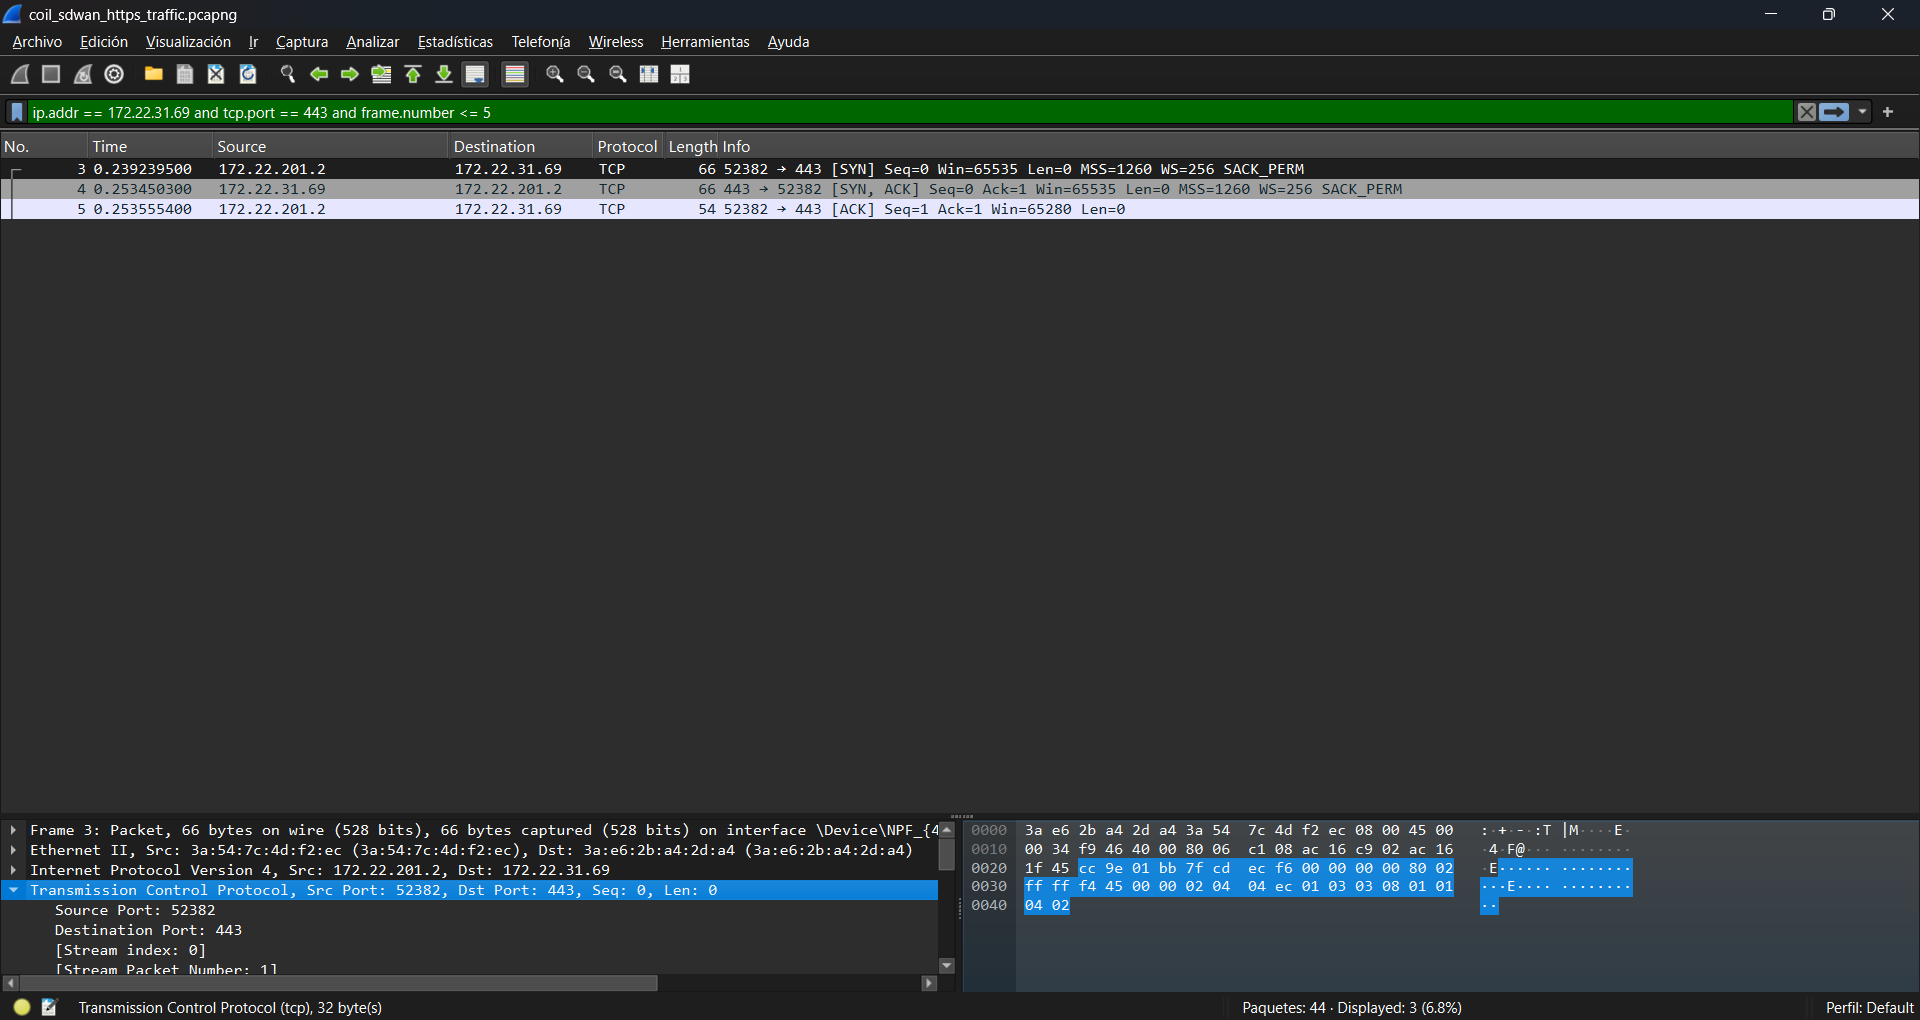
\includegraphics[width=0.94\textwidth]{figuras/wireshark_2_tcp_handshake.png}
    \caption{Wireshark packet details for the initial TCP three-way handshake (Frames~3--5), confirming \texttt{MSS=1260} matching the \qty{1300}{\byte} ZeroTier MTU minus \qty{40}{\byte} IPv4/TCP headers, \texttt{WS=256} scaling to \texttt{Win=65280}, \texttt{SACK\_PERM}, and a \qty{14.21}{\milli\second} handshake RTT.}
    \label{fig:ws_handshake}
\end{figure*}

\subsection{TLS 1.3 Cryptographic Handshake and Encrypted HTTP/1.1 Payload Transfer}
\label{subsec:ws_tls}

Immediately following TCP synchronization, Frames~6--35 execute the RFC~8446 TLS~1.3 handshake and encrypted application-layer exchange~\cite{rfc8446}, illustrated in Fig.~\ref{fig:ws_tls} and traced in Fig.~\ref{fig:tcp_tls_sequence}:
\begin{itemize}
    \item \textbf{Segmented Client Hello (Frames~6--7, \qty{0.2543708}{\second}):} The client initiates cryptographic negotiation with a \texttt{Client Hello} carrying Server Name Indication (\texttt{SNI=www.coil-group2.com}), \texttt{supported\_versions} (\texttt{TLS 1.3}), three AEAD cipher suites---\texttt{0x1302} (\nolinkurl{TLS_AES_256_GCM_SHA384}), \texttt{0x1303} (\nolinkurl{TLS_CHACHA20_POLY1305_SHA256}), and \texttt{0x1301} (\nolinkurl{TLS_AES_128_GCM_SHA256})---and an extended \texttt{key\_share} payload offering hybrid post-quantum \texttt{X25519MLKEM768} alongside \texttt{x25519}. Because the resulting \qty{1479}{\byte} TCP payload exceeds the \qty{1260}{\byte} MSS, TCP segments the message into Frame~6 (\qty{1260}{\byte} payload) and Frame~7 (\qty{219}{\byte} payload), which Wireshark reassembles ($1260 + 219 = \qty{1479}{\byte}$) into the complete \texttt{Client Hello} record.
    \item \textbf{Single-RTT Server Flight (Frames~9--12, \qty{0.2732436}{\second}):} After acknowledging Frame~7 (\texttt{Ack=1480} in Frame~8), the server responds in a single round trip across Frames~9--12 (\qty{2900}{\byte} TLS handshake flight). Frame~9 begins with \texttt{Server Hello}, selecting cipher suite \texttt{0x1302} (\nolinkurl{TLS_AES_256_GCM_SHA384}) and \texttt{x25519} key agreement, followed immediately by a middlebox-compatibility \texttt{Change Cipher Spec} record and encrypted handshake records spanning Frames~9, 10, and 12 (\texttt{Encrypted Extensions}, the X.509 certificate chain anchored to \texttt{COIL Group 2 Root CA}, \texttt{CertificateVerify}, and \texttt{Finished}).
    \item \textbf{Encrypted HTTP/1.1 Transaction (Frames~13--35, \qty{0.2744180}{\second}--\qty{0.3358339}{\second}):} At \qty{0.2744180}{\second} (Frame~13, \qty{80}{\byte} TCP payload), the client emits \texttt{Change Cipher Spec} plus its encrypted \texttt{Finished} message; the server issues post-handshake session tickets in Frames~14 and~16 (\qty{255}{\byte} TCP payload each). In Frame~15 (\qty{0.2874402}{\second}, \qty{178}{\byte} wire), the client transmits the encrypted HTTP \texttt{GET /seneca/} request inside a \qty{124}{\byte} TLS application-data payload (\texttt{Seq=1560..1683}). The server then delivers the HTTP \texttt{200 OK} headers and the full \qty{15470}{\byte} HTML document (\qty{15734}{\byte} decrypted HTTP bytes total) across Frames~17--35. Consistent with the negotiated \texttt{MSS=1260}, bulk server segments (Frames~17, 19--20, 22--23, 25--26, 28--29, 31--32, and~34) each carry exactly \qty{1260}{\byte} of encrypted payload (\qty{1314}{\byte} wire), while the final application record in Frame~35 (\qty{658}{\byte} payload) advances the server's relative sequence space to \texttt{Seq=19136}.
\end{itemize}

Because all HTTP headers and HTML markup after \texttt{Server Hello} and client \texttt{Finished} appear strictly as opaque TLS~1.3 \texttt{Application Data} in Fig.~\ref{fig:ws_tls}, passive observers on either the underlay network or the virtual broadcast domain cannot recover payload content or tamper with responses without failing AEAD authentication~\cite{rfc8446}.

\begin{figure*}[t]
    \centering
    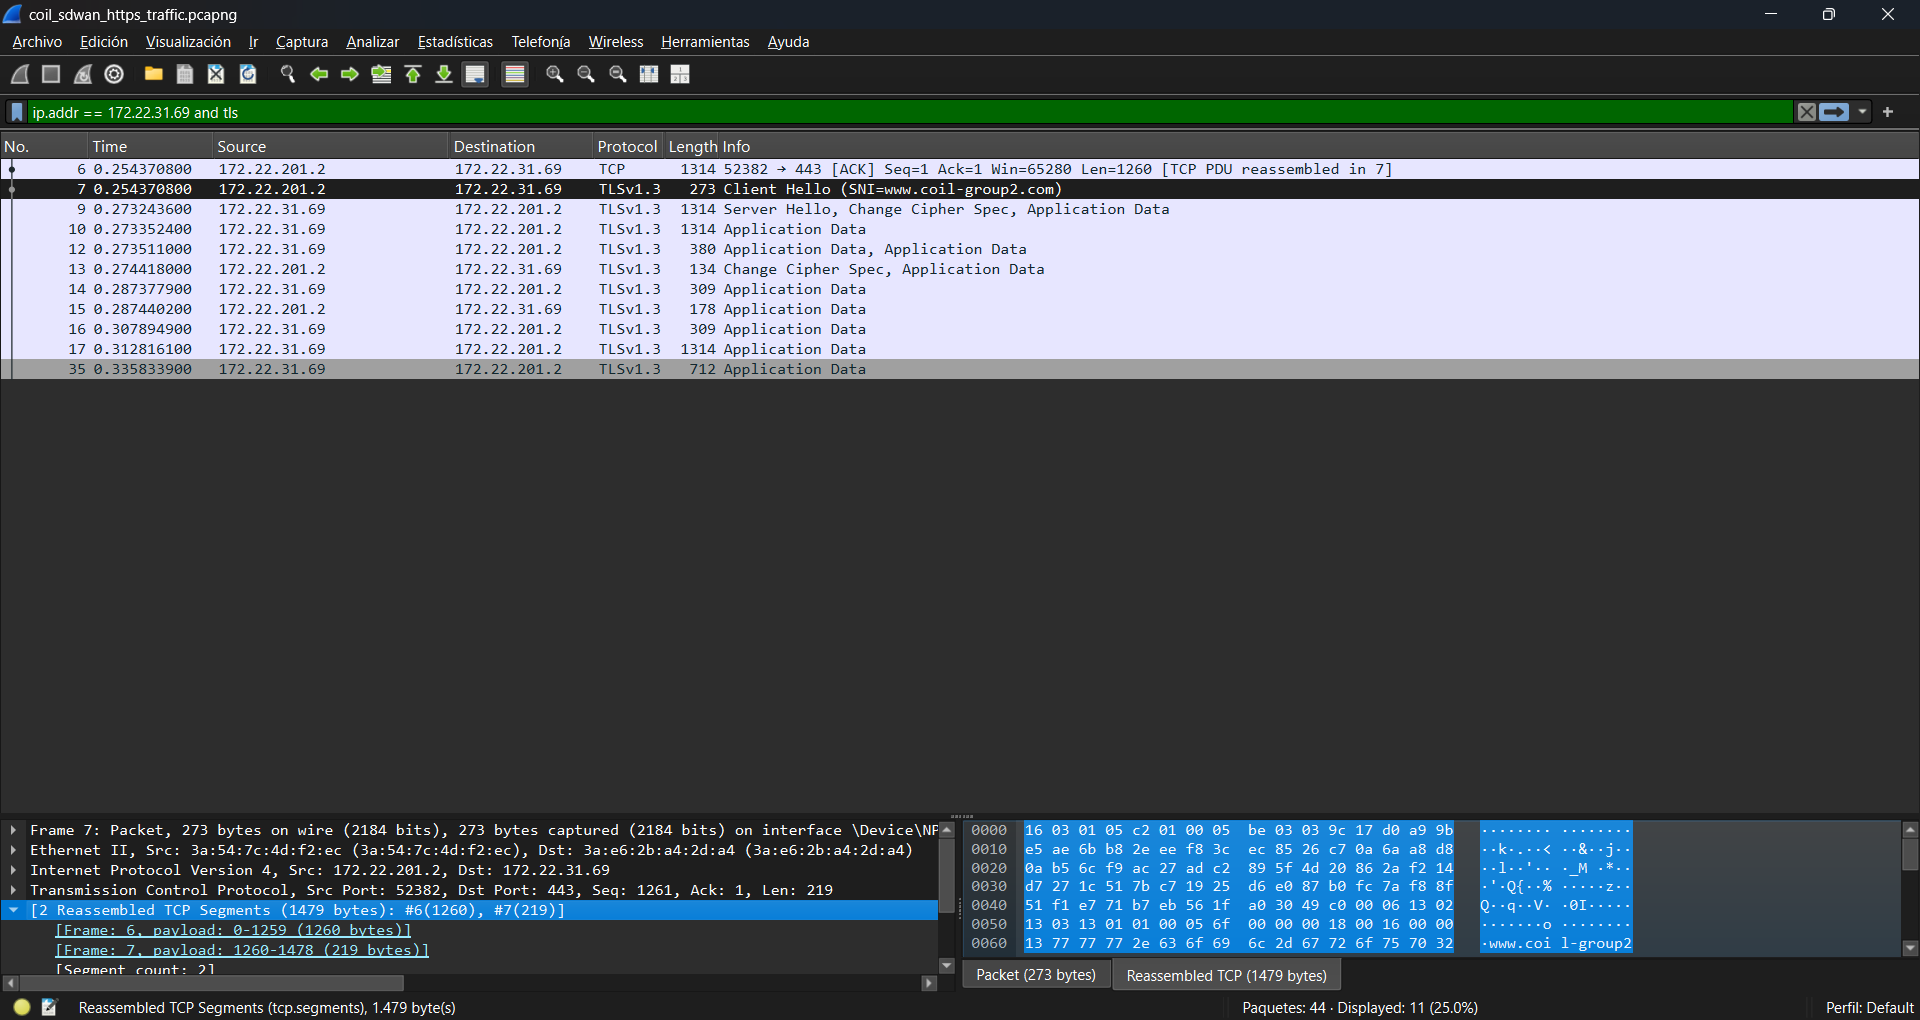
\includegraphics[width=0.94\textwidth]{figuras/wireshark_3_tls_data_exchange.png}
    \caption{Wireshark inspection of the TLS~1.3 cryptographic handshake and encrypted HTTP/1.1 payload exchange (Frames~6--35), showing reassembled \texttt{Client Hello} (\texttt{SNI=www.coil-group2.com}), 1-RTT \texttt{Server Hello} selecting \texttt{TLS\_AES\_256\_GCM\_SHA384} (\texttt{0x1302}), and \qty{1260}{\byte}-MSS segmented delivery of the \qty{15470}{\byte} Seneca HTML response.}
    \label{fig:ws_tls}
\end{figure*}

\subsection{Graceful TCP Connection Teardown}
\label{subsec:ws_teardown}

Once the Seneca HTML payload is transmitted, the server closes the connection cleanly in accordance with HTTP/1.1 \texttt{Connection: close} header semantics and RFC~9293 finite-state termination~\cite{rfc9293,kozierok2005}. Fig.~\ref{fig:ws_teardown} highlights the final four teardown frames (Frames~35--38, corresponding to the bottom phase of Fig.~\ref{fig:tcp_tls_sequence}):
\begin{enumerate}
    \item \textbf{Frame~35 (\qty{0.3358339}{\second}, \qty{712}{\byte} wire):} The server piggybacks \texttt{[FIN, PSH, ACK]} onto the concluding \qty{658}{\byte} encrypted payload segment (\texttt{Seq=18477}, \texttt{Ack=1684}, \texttt{Len=658}), incrementing its cumulative sequence boundary by $658 + 1 = 659$ to \num{19136}.
    \item \textbf{Frame~36 (\qty{0.3359537}{\second}, \qty{54}{\byte} wire):} Within \qty{0.1198}{\milli\second}, the client transmits \texttt{[ACK]} (\texttt{Seq=1684}, \texttt{Ack=19136}, \texttt{Len=0}), acknowledging both the trailing payload bytes and the server's \texttt{FIN} flag to close the server-to-client half-channel.
    \item \textbf{Frame~37 (\qty{0.6367030}{\second}, \qty{54}{\byte} wire):} Upon completing local socket shutdown, the client issues \texttt{[FIN, ACK]} (\texttt{Seq=1684}, \texttt{Ack=19136}, \texttt{Len=0}) to close its own transmit half-channel.
    \item \textbf{Frame~38 (\qty{0.6475791}{\second}, \qty{54}{\byte} wire):} The server confirms termination with \texttt{[ACK]} (\texttt{Seq=19136}, \texttt{Ack=1685}, \texttt{Len=0}), cleanly retiring the session at \qty{0.4083}{\second} elapsed stream time.
\end{enumerate}

Verification against the display filter \texttt{tcp.flags.reset == 1} confirms \textbf{zero \texttt{RST} flags} across the entire capture file. The absence of forced resets proves that both TLS~1.3 session closure and HTTP/1.1 socket release operated deterministically without protocol errors or premature peer aborts.

\begin{figure*}[t]
    \centering
    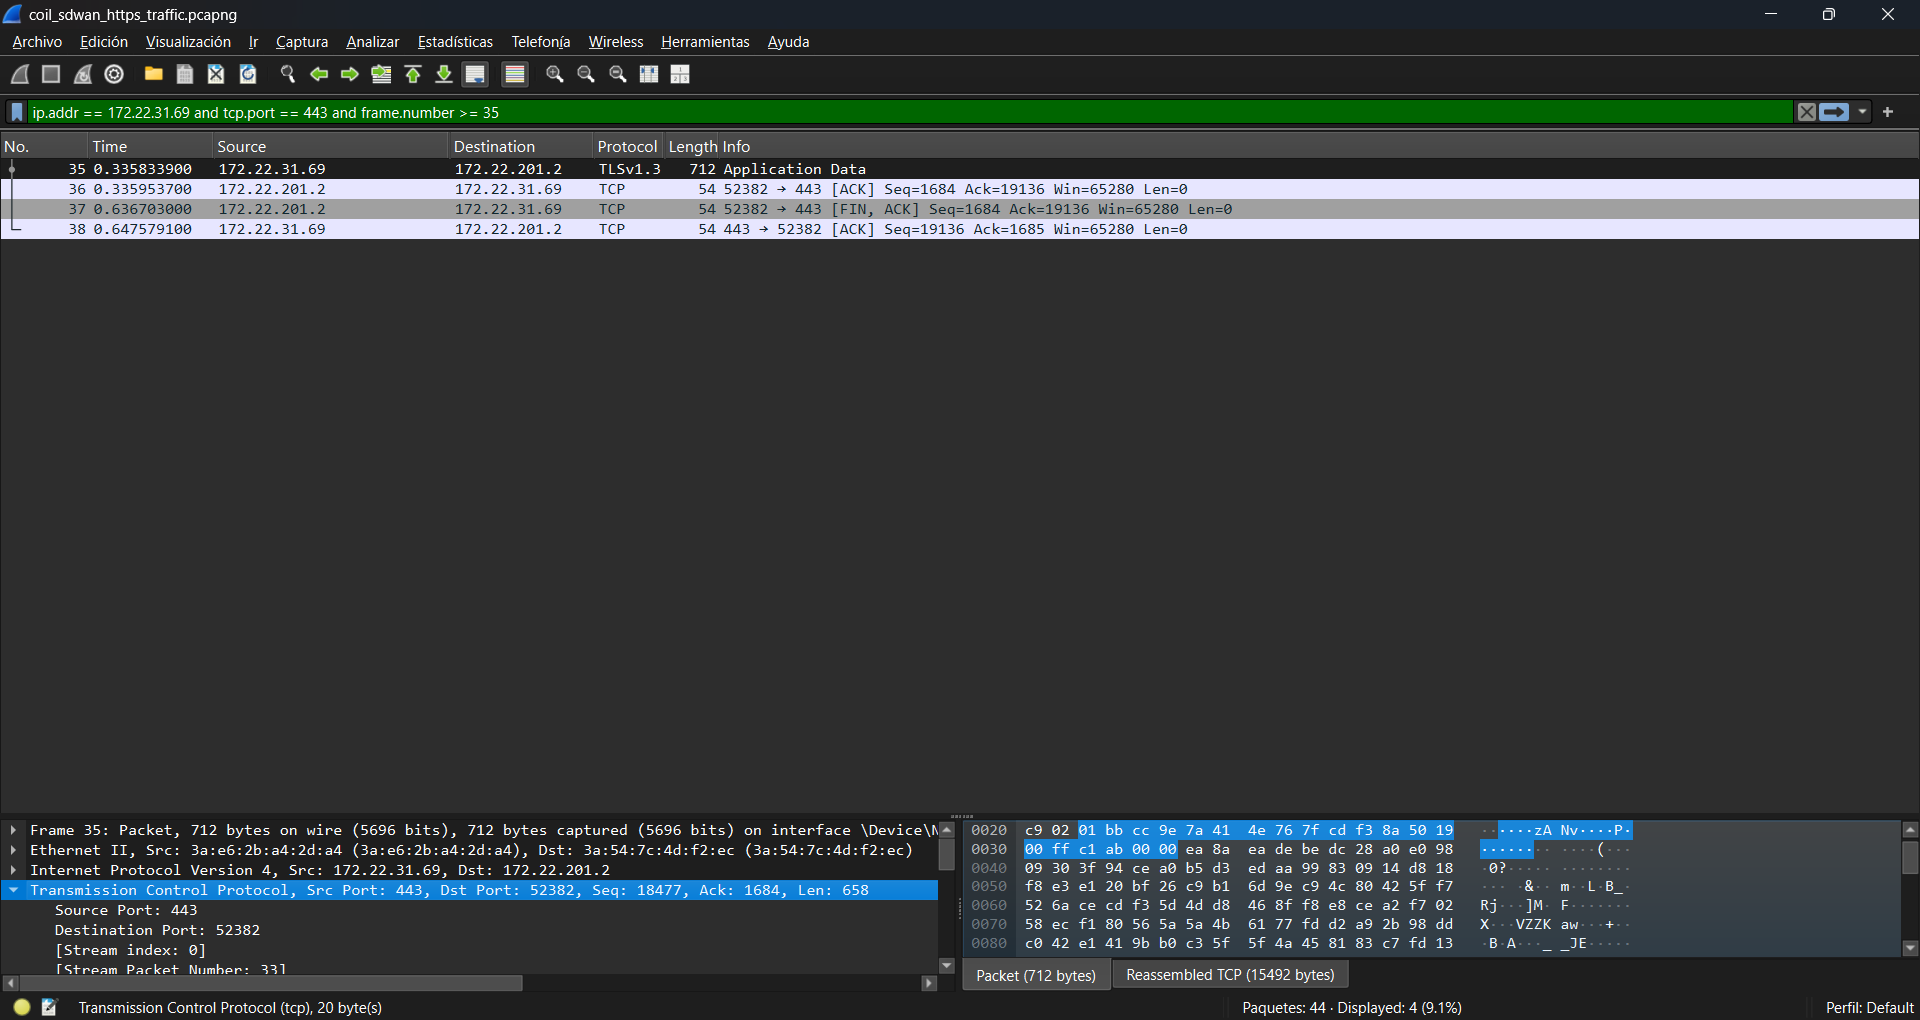
\includegraphics[width=0.94\textwidth]{figuras/wireshark_4_tcp_teardown.png}
    \caption{Wireshark inspection of the clean four-way TCP connection teardown (Frames~35--38), showing server \texttt{[FIN, PSH, ACK]} (\texttt{Seq=18477, Ack=1684, Len=658}), client \texttt{[ACK]} (\texttt{Ack=19136}), client \texttt{[FIN, ACK]}, and final server \texttt{[ACK]} (\texttt{Ack=1685}) with zero \texttt{RST} packets.}
    \label{fig:ws_teardown}
\end{figure*}
